\chapter{Introduction}

Alkemics is a start-up that was founded in 2011. Back then, they created e-merchandising tools to improve user experience on e-commerce websites. It then evolved to become a platform that enables the FMCG (Fast-Moving Consumer Goods) ecosystem to share all their data, from product to transactional information, in order to improve pricing, supply, marketing.

Alkemics develops products that enable collaboration between Brands and Retailers, and tackle the challenges of omni-channel commerce and smart customer interaction.

\section{Alkemics}

\begin{figure}[H]
\centering
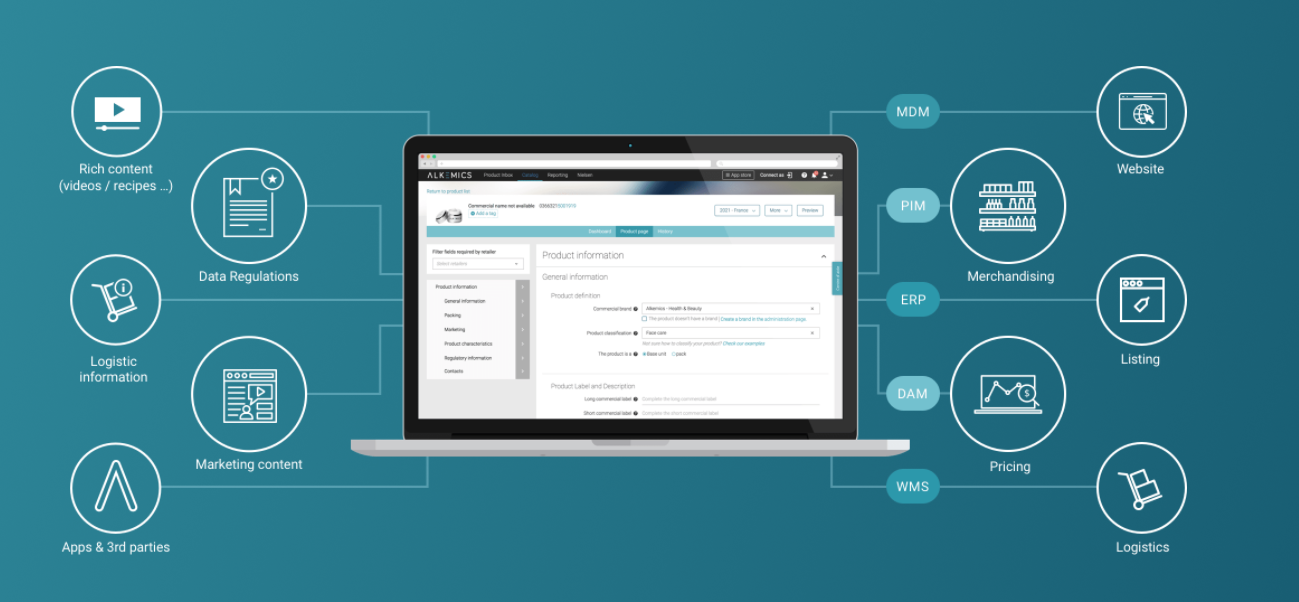
\includegraphics[scale=0.30]{./images/alkemics_website_global.png}
\caption{Alkemics}
\end{figure}

\subsection{Product Data Empowerment}

Because of increasing regulations, new customer demands, omni-channel communications, there is a growing need for richer and more exhaustive product information as well as an exponentially growing number of products. Some products change more than 10 times per year (promotion, seasonality, new recipes, new packagings...), and overall, 40\% of products are renewed every year.

This cascades in a series of problems that handicap manufacturers, retailers and consumers: logistics struggle to maintain stock, accounting systems fail to track how different products are actually the same consumption unit, pricing teams struggle to maintain price coherency in this dynamic environment, marketing teams are inefficient to share richer and richer content about the product, BI teams feel that the consumption of the consumer are changing while they actually don't.

This problem is called product chaining. It describes the ability to connect products that share a given set of attributes in order to understand how they relate.

To overcome these problems, Alkemics built a product taxonomy reinforced by an ontology. PDE \footnote{Product Data Empowerment} team is fully dedicated to enhance the classification task to automatically classify the category of products, as well as the brand and other attributes such as the packaging or the price range. The classification task mainly uses Natural Language Processing techniques and distances in semantic spaces. PDE is also in charge of the management of the product data model.


\subsection{Product Stream}

Product Stream is a web application that enables:
\\

\textbf{Makers} to:
    \begin{itemize}
    \item Collect product information from all the stakeholders of the organization: the \textit{supply team} who knows the size and weight of the product, the \textit{marketing team} who owns the pictures, videos as well as the brand content, the \textit{quality team} who masters the composition, nutritional values, etc.
    \item Store product information in a centralized way, so everyone in the organization can have access to it (DAM \footnote{Digital Asset Management}).
    \item Distribute product information so every partner has the same up-to-date information. This includes retailers, but also marketing agencies, trade marketing agencies, ... (EDI \footnote{Electronic Data Interchange} / PIM \footnote{Product information management})
    \item Collaborate with 3rd parties to collect user reviews,  receive data quality reports,  print coupons, use buy-it-now solutions.
    \end{itemize}

\textbf{Retailers} to:
    \begin{itemize}
    \item Have access to best-in-class product information to power their tools and feed their digital supports (EDI)
    \item Collaborate with manufacturers to reference new products \& innovations, run call-for-proposals for promotional formats, etc…
    \item Connect products that share a given set of attributes in order to understand how they relate (Product Chaining).
    \end{itemize}

\subsection{The technological stack}

\textbf{Micro-services architecture}
The stack in Alkemics is composed of set of dozens of micro services communicating with synchronous calls (HTTPS) and both synchronous and asynchronous messaging (TCP enabled by Rabbit MQ).
Each service has a domain specific task: data ingestion, data classification, APIs for merchandising, etc. A subset of the services are exposed to third parties and clients.

\textbf{User interface}
User Interface dashboards also call the APIs to make functionalities available to the users (makers and retailers) trough a web browser.
The front part of the website is implemented with React framework.

\textbf{APIs and SDKs}
A set of SDKs are also provided to retailers to allow them to use merchandising functionalities directly embedded in their websites.

\textbf{Storage vs indexation}
All Alkemics crucial data is stored in relational databases (MySQL). Yet if relationnal databases provide very useful functionalities to guaranty integrity of data, its indexing capabilities remain quite poor in comparison to non-relational databases.

That's we also create ElasticSearch indexes, containing data that is already stored in relational databases, but indexed in a format allowing quick and performant queries.


\section{Professional thesis objective}

This professional thesis aims at implementing machine learning techniques to improve products data quality.
